%!TEX root = ../main.tex

\section{Poisson-disk sampling of the depthmap}
\label{sec:poisson_sampling}

In semi-regular triangle remeshing, to construct a semi-regular mesh from an irregular one, one method consists in constructing a base mesh, i.e. a low resolution version of the irregular one, subdividing its triangles recursively and projecting the generated vertices onto the original surface \cite{PRS15}. Our work is inspired by those methods, constructing first a base mesh in 2D from a set of samples on the surface, i.e pixels on the depthmap, and then reconstructing the different levels of resolution by recursive subdivision.

To obtain a good distribution of the base vertices over the depthmap, we use a poisson-disk sampling \cite{Coo86}, as it has been shown to be one of the best sampling patterns for many applications. 
We use a dart-throwing approach to choose the samples, combined with an region-growing process through Dijkstra's algorithm \cite{Dij59} to compute the disks areas.
We compute a connectivity graph over the depthmap. Each pixel can have up to 6 neighbors, with respect to the triangulation pattern chosen at the beginning (Fig. \ref{fig:pixel_neighborhood}).
An edge is created between every pair of neighboring pixels if they belong to the same surface area, meaning that they are not separated by a border. 
The weight of each edge is chosen depending on the metric considered.

\subsection{Uniform sampling}
This method uses the 3D coordinates of points (where each point is a pixel embedded in 3D using the depth information stored at that pixel) and weights each edge using the euclidean distance between both points sharing this edge.
By using Dijkstra's algorithm, we can then construct the shortest path between a source (center of a disk) and any point of the domain.
By using this method, we consider Poisson disks (surface patches to be more precise) that have an uniform area in 3D.

\begin{figure}[ht]
\centering
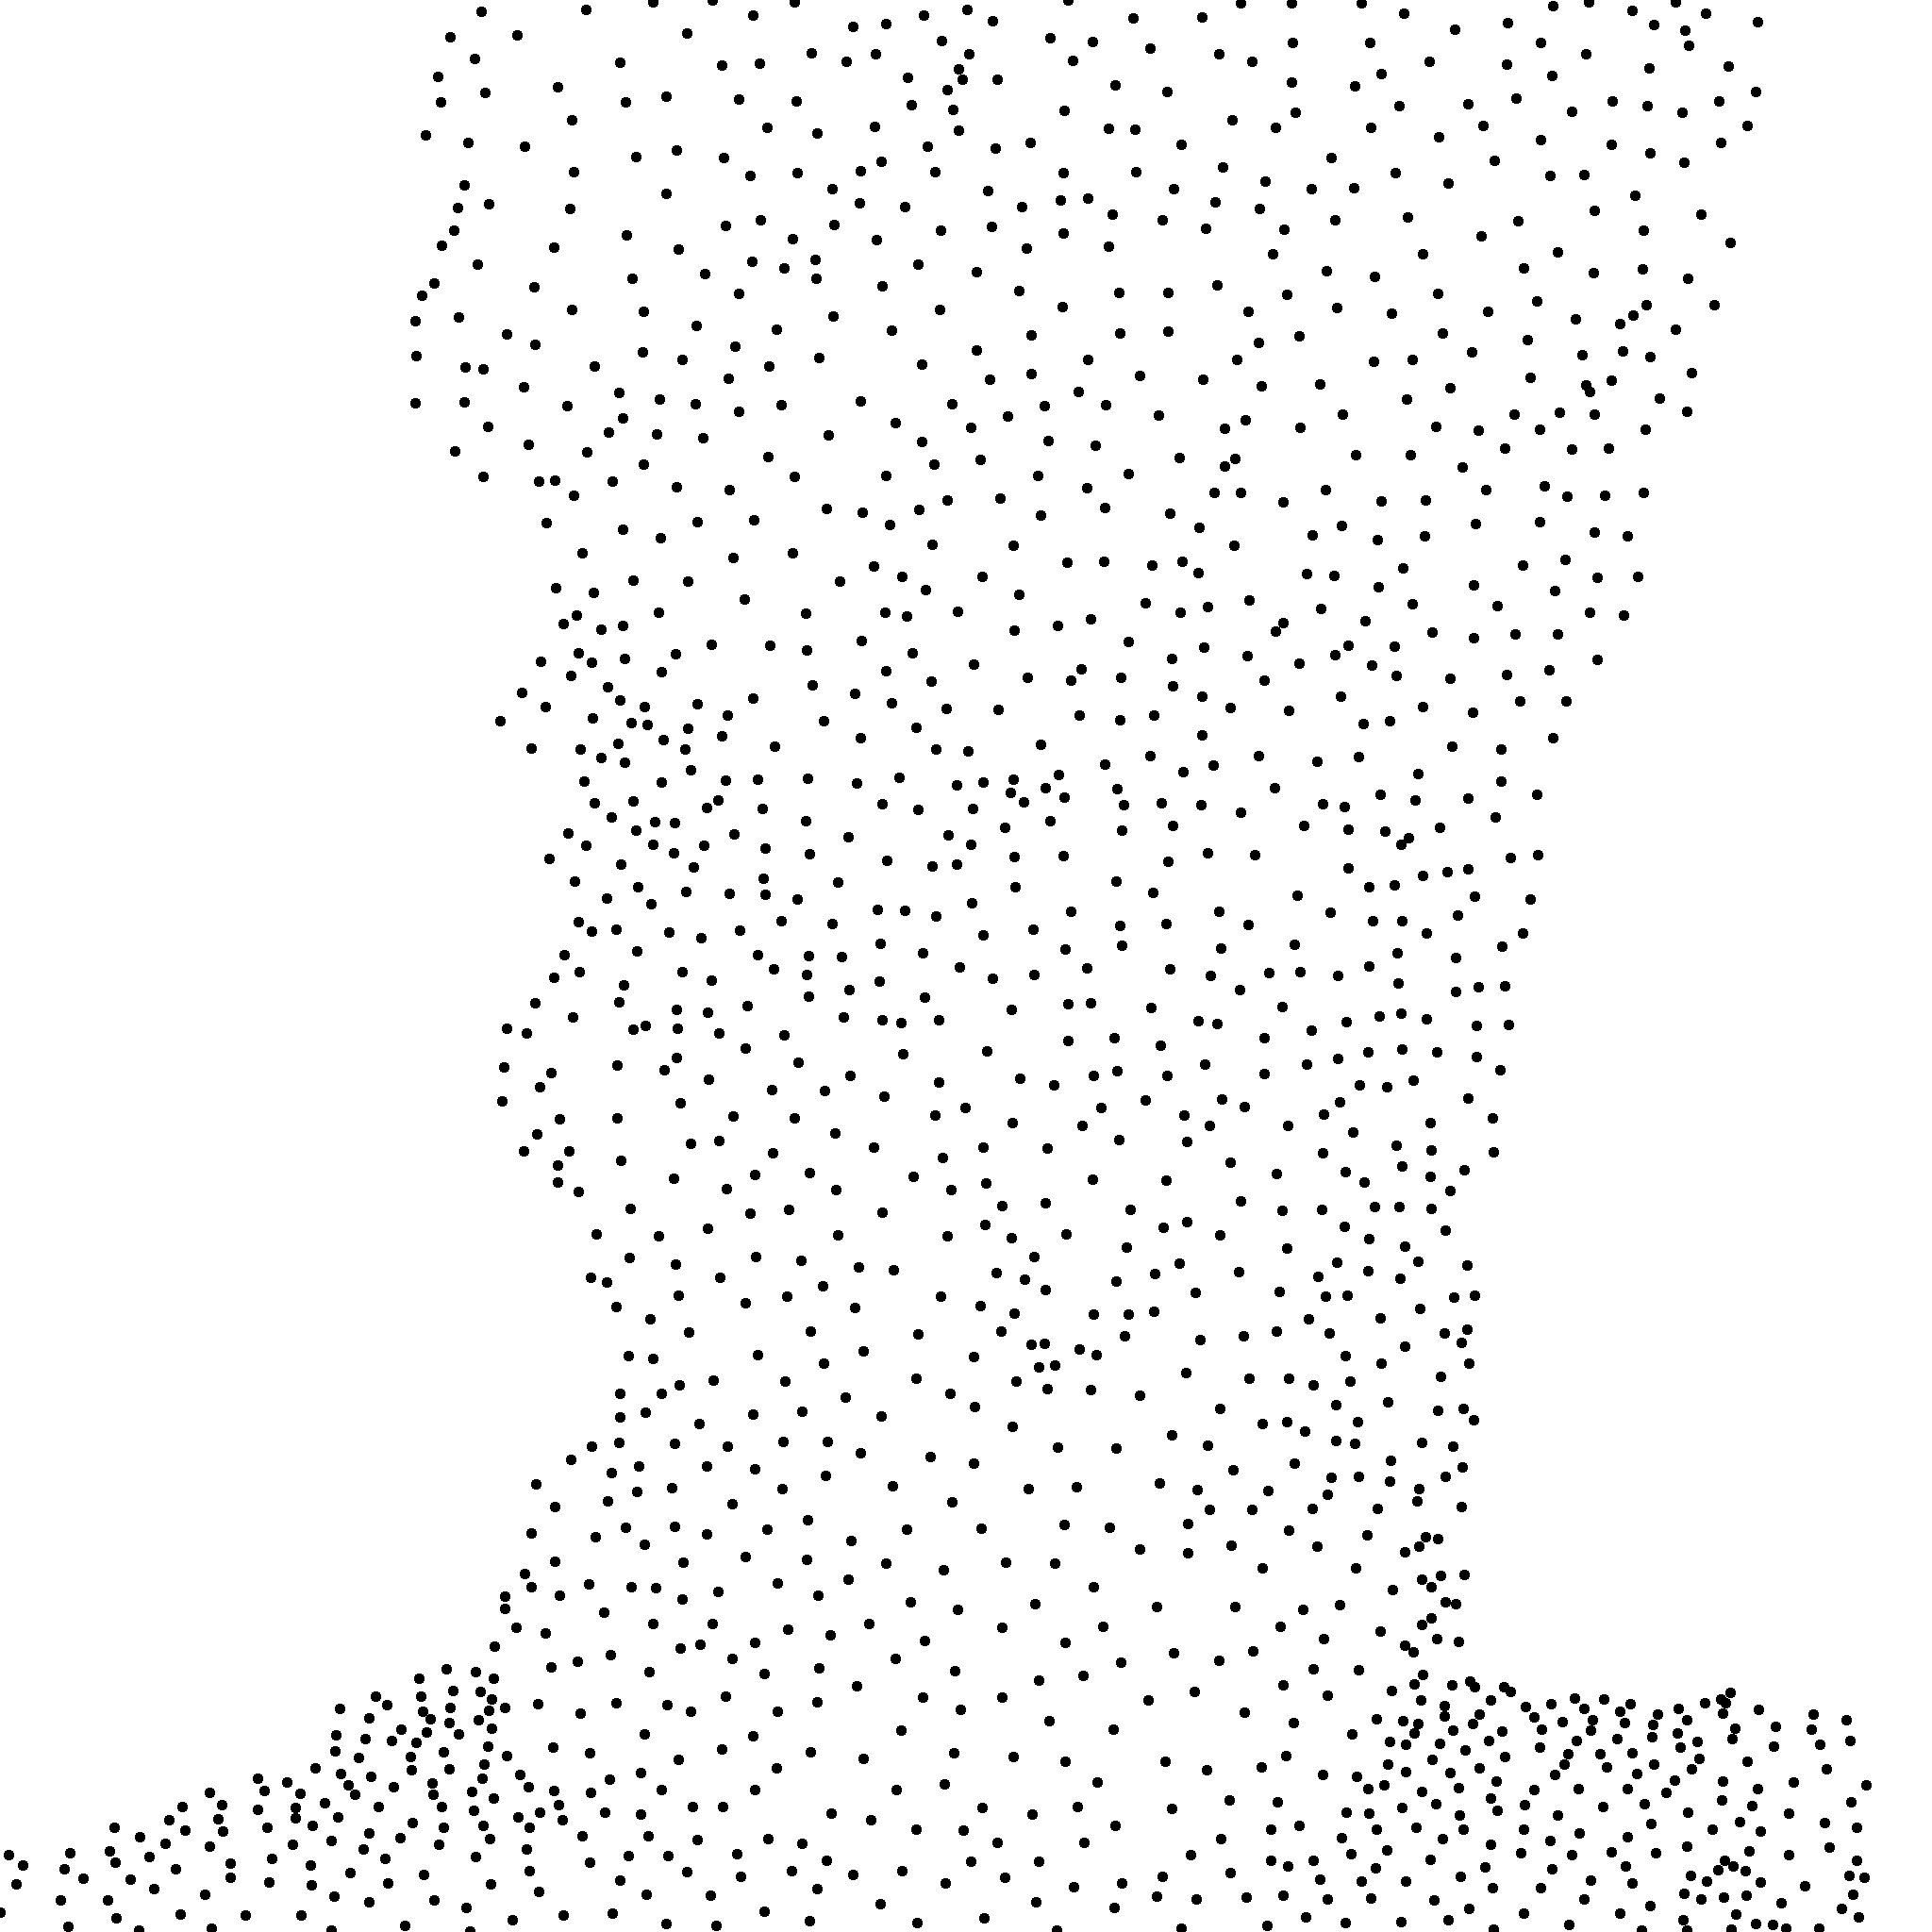
\includegraphics[scale=0.05]{PoissonSampling3D-Garuda}
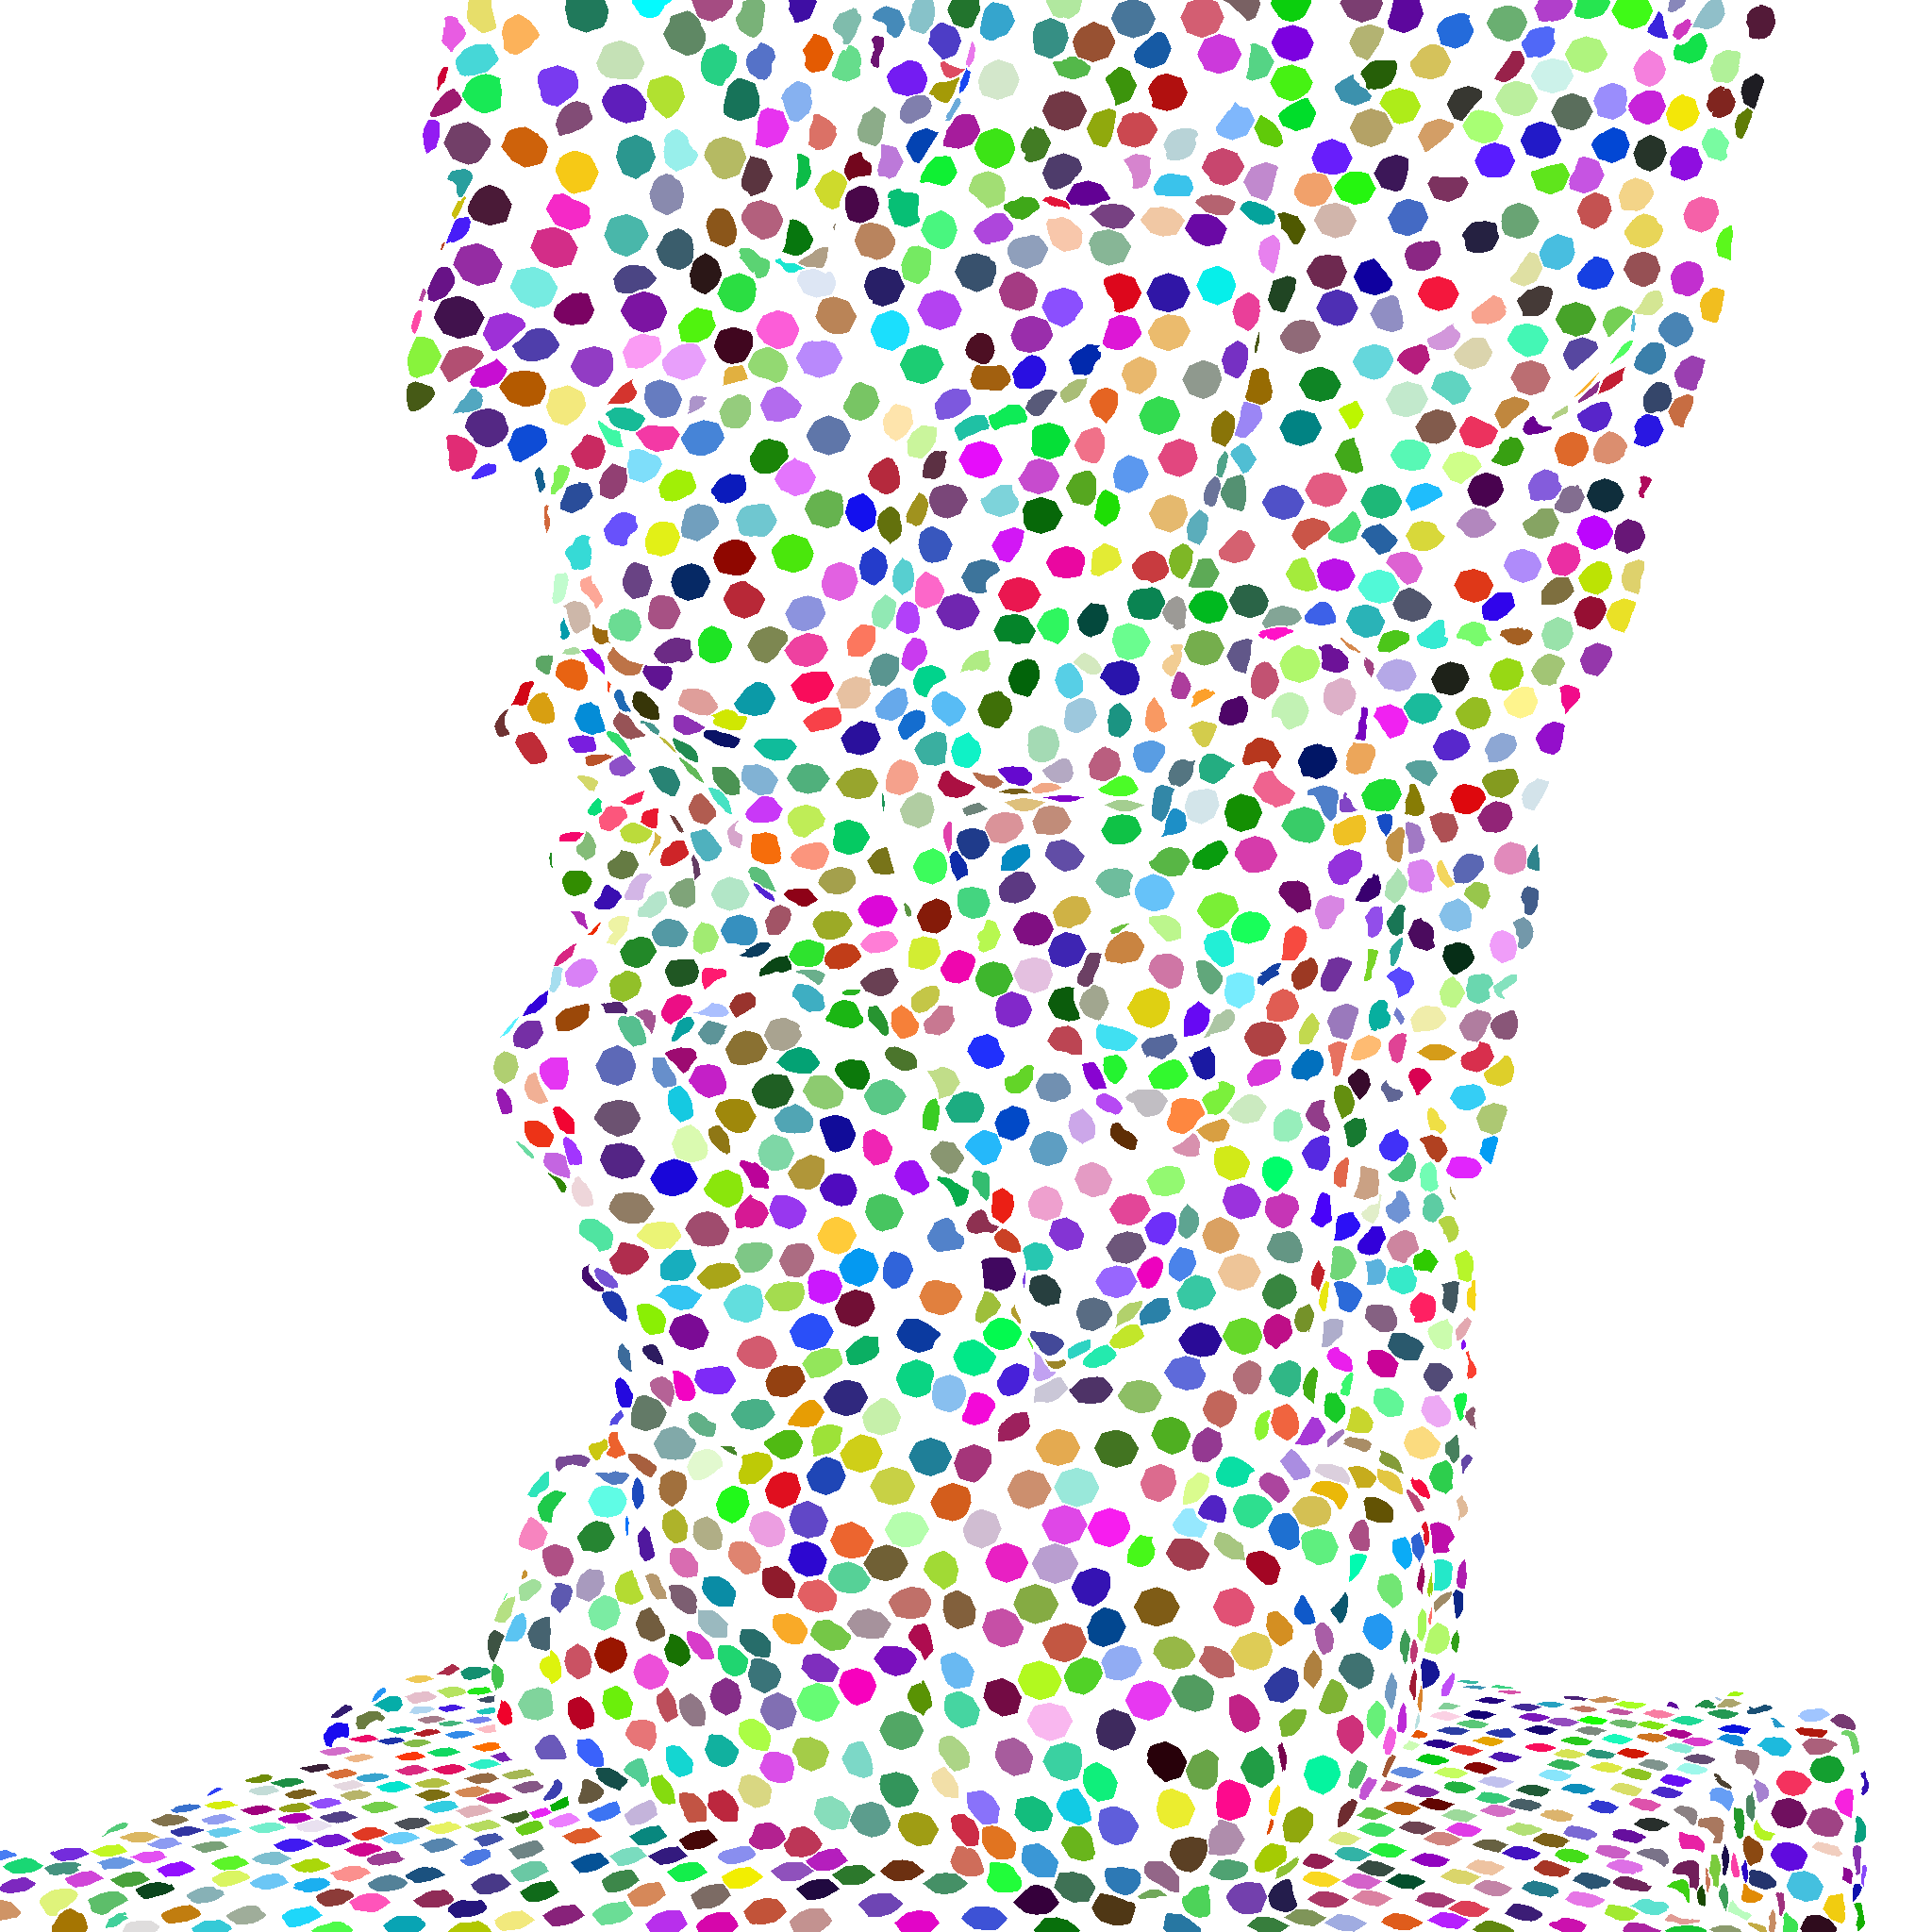
\includegraphics[scale=0.05]{PoissonDisks3D-Garuda}
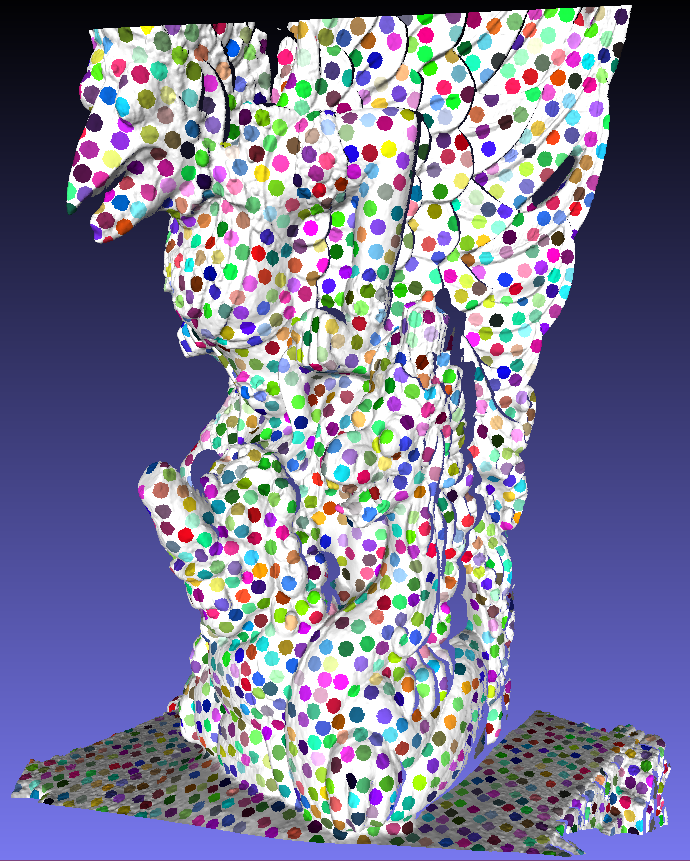
\includegraphics[scale=0.12]{PoissonDisks3DEmbedded-Garuda}
\caption{Poisson-disk sampling of the Garuda model considering disks with an uniform area in 3D (a) with their associated disks (b) and the same disks, but embedded in 3D (c)}
\label{fig:poisson_sampling_3d}
\end{figure}

\subsection{Density adaptive sampling}
Depthmaps can represent scenes having a really huge difference in sampling density, depending on the distance of a surface area to the scanner. 
For example, on the (Figure \arnaud{ADD FIGURE SHOWING THE SAMPLING DENSITY DIFFERENCE}) points in the green area have a sampling density of \arnaud{sampling density value w.r.t Bbox} and the pixels in the blue area have a sampling density of \arnaud{sampling density value w.r.t Bbox}. It can be interesting to conserve that difference of density when choosing the samples, in order to keep the precision of the original acquisition, when fine structures have been acquired.

Instead of sampling a point cloud uniformly in 3D, we suggest to take the local sampling density into account. In other words, rather than computing disks with an uniform radius in 3D, we constrain each disk to have an uniform radius in 2D.
Interestingly, this can easily be obtained by sampling the depthmap without considering 3D geodesic distances, i.e. doing a classical Poisson-disk sampling on an discretized planar domain, using a Dart Throwing approach for example.

\begin{figure}[ht]
\centering
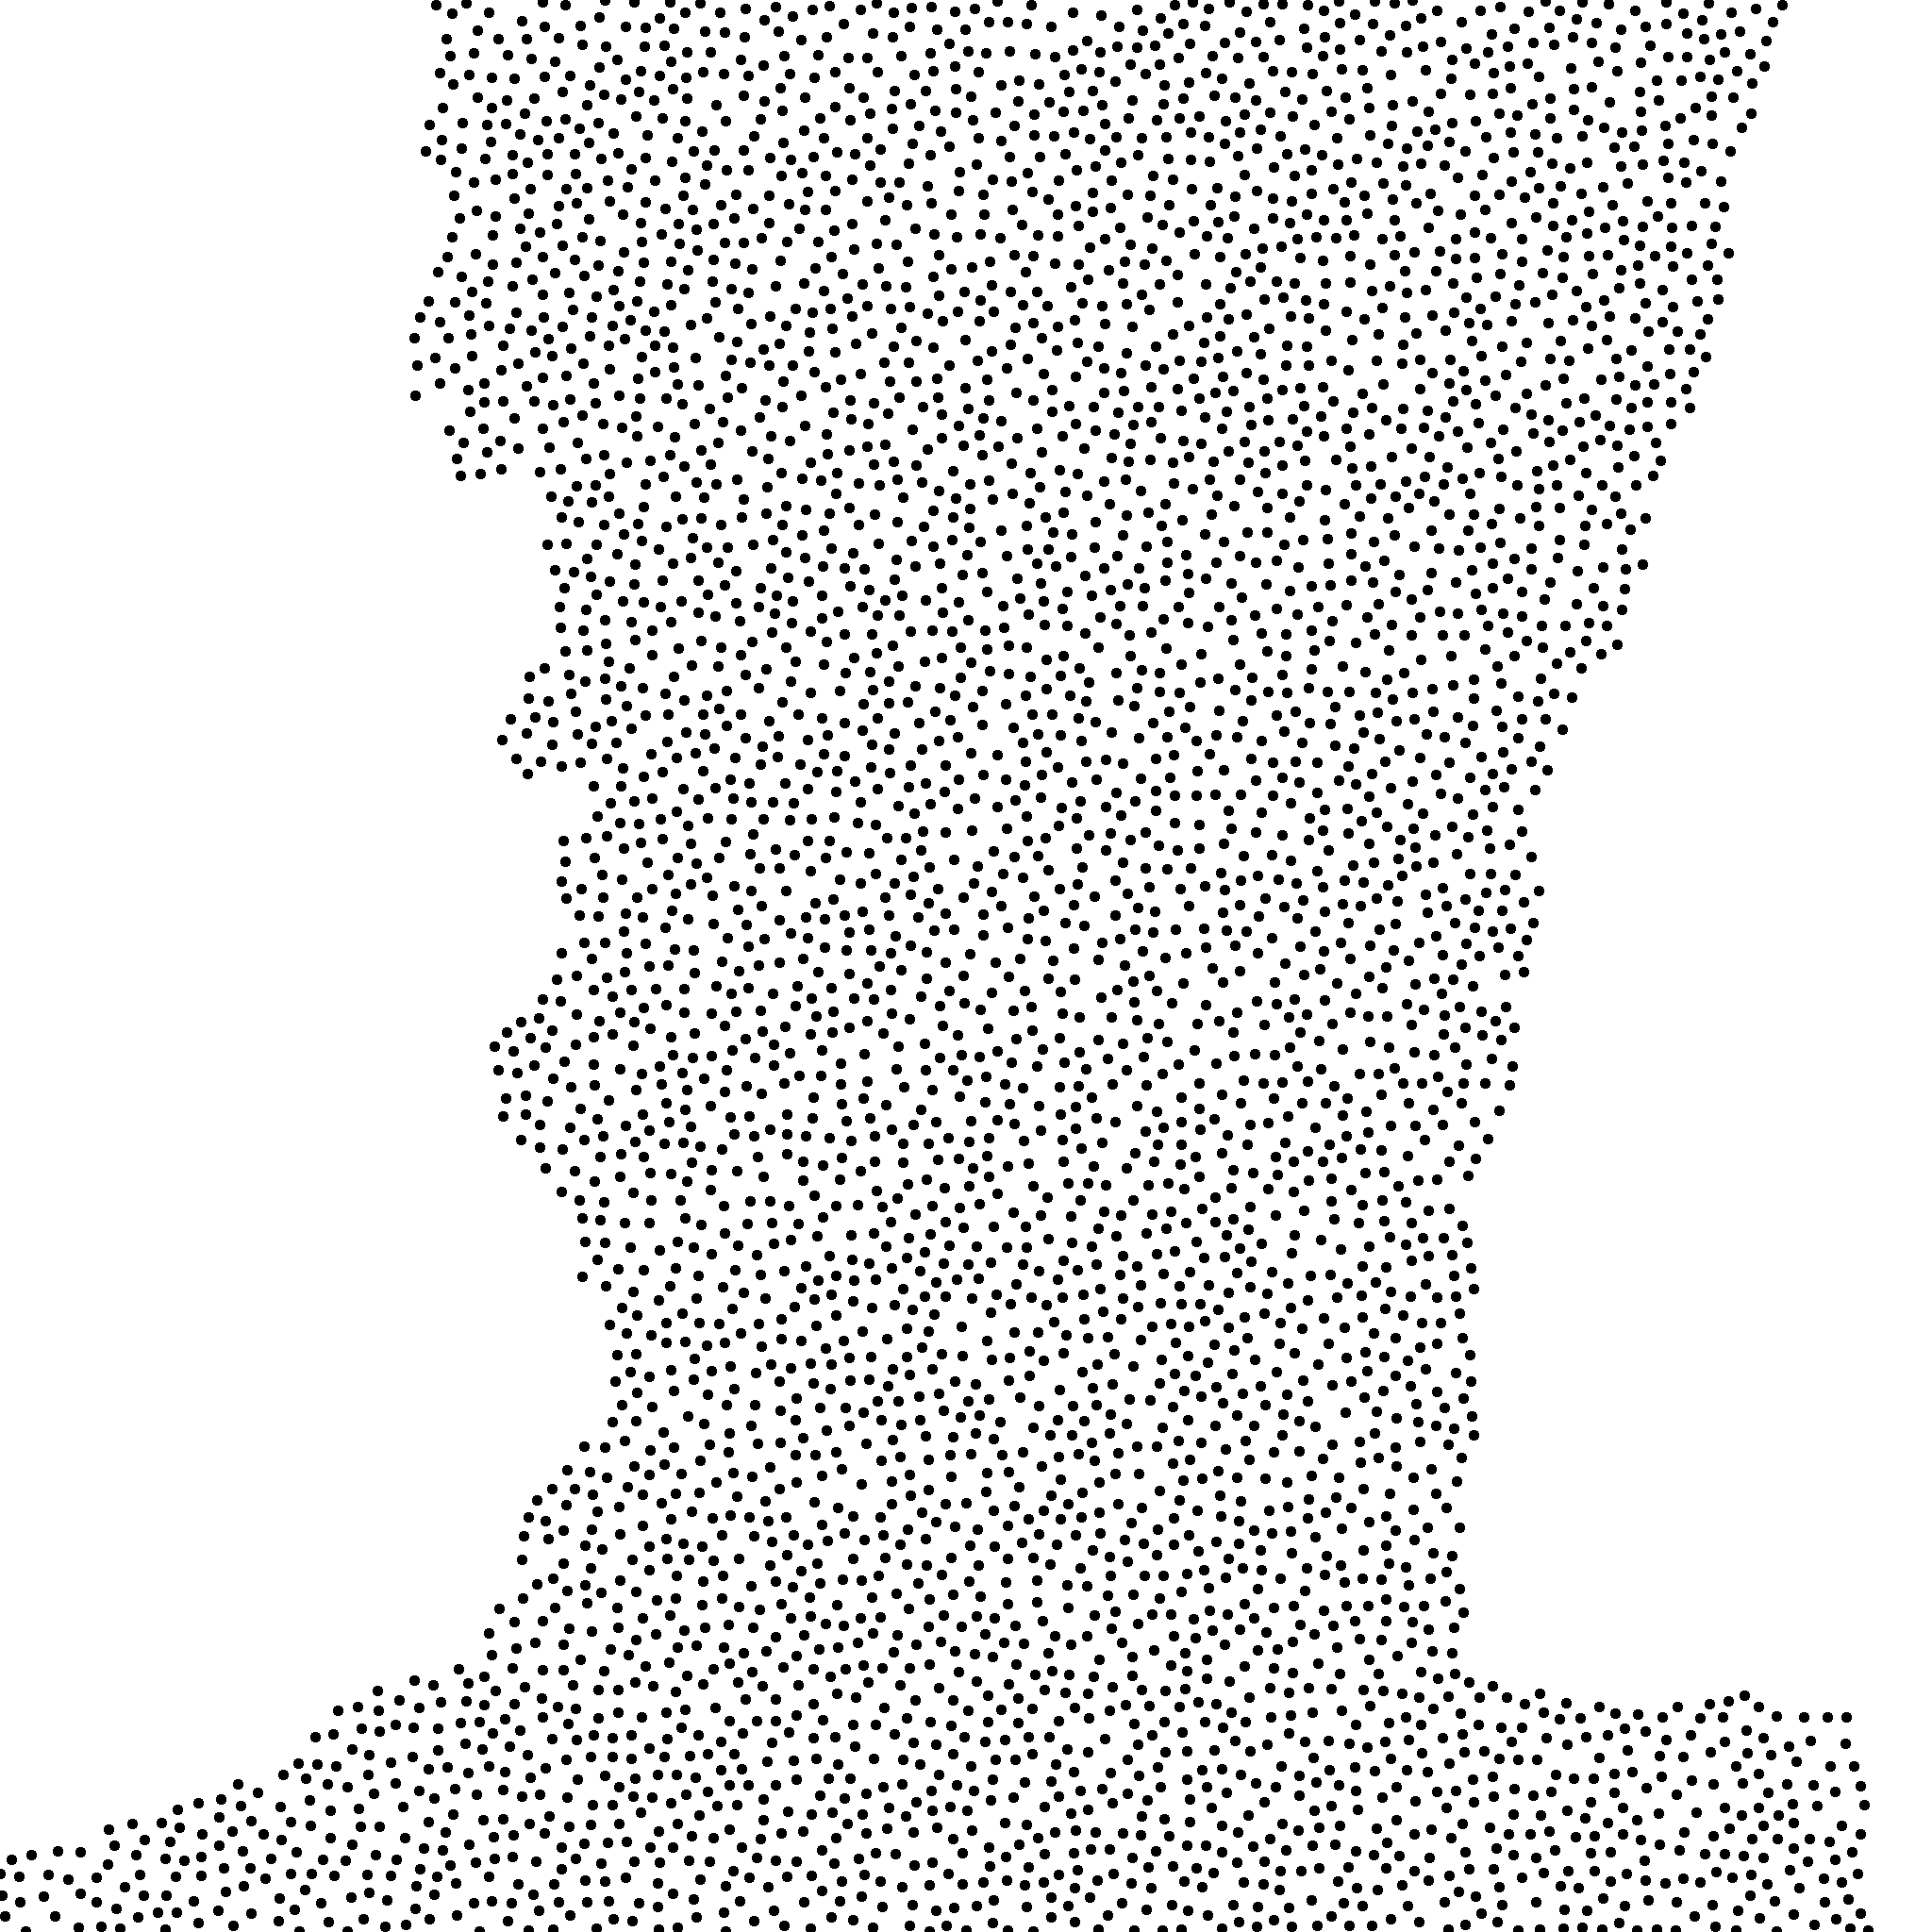
\includegraphics[scale=0.06]{PoissonSampling2D-Garuda}
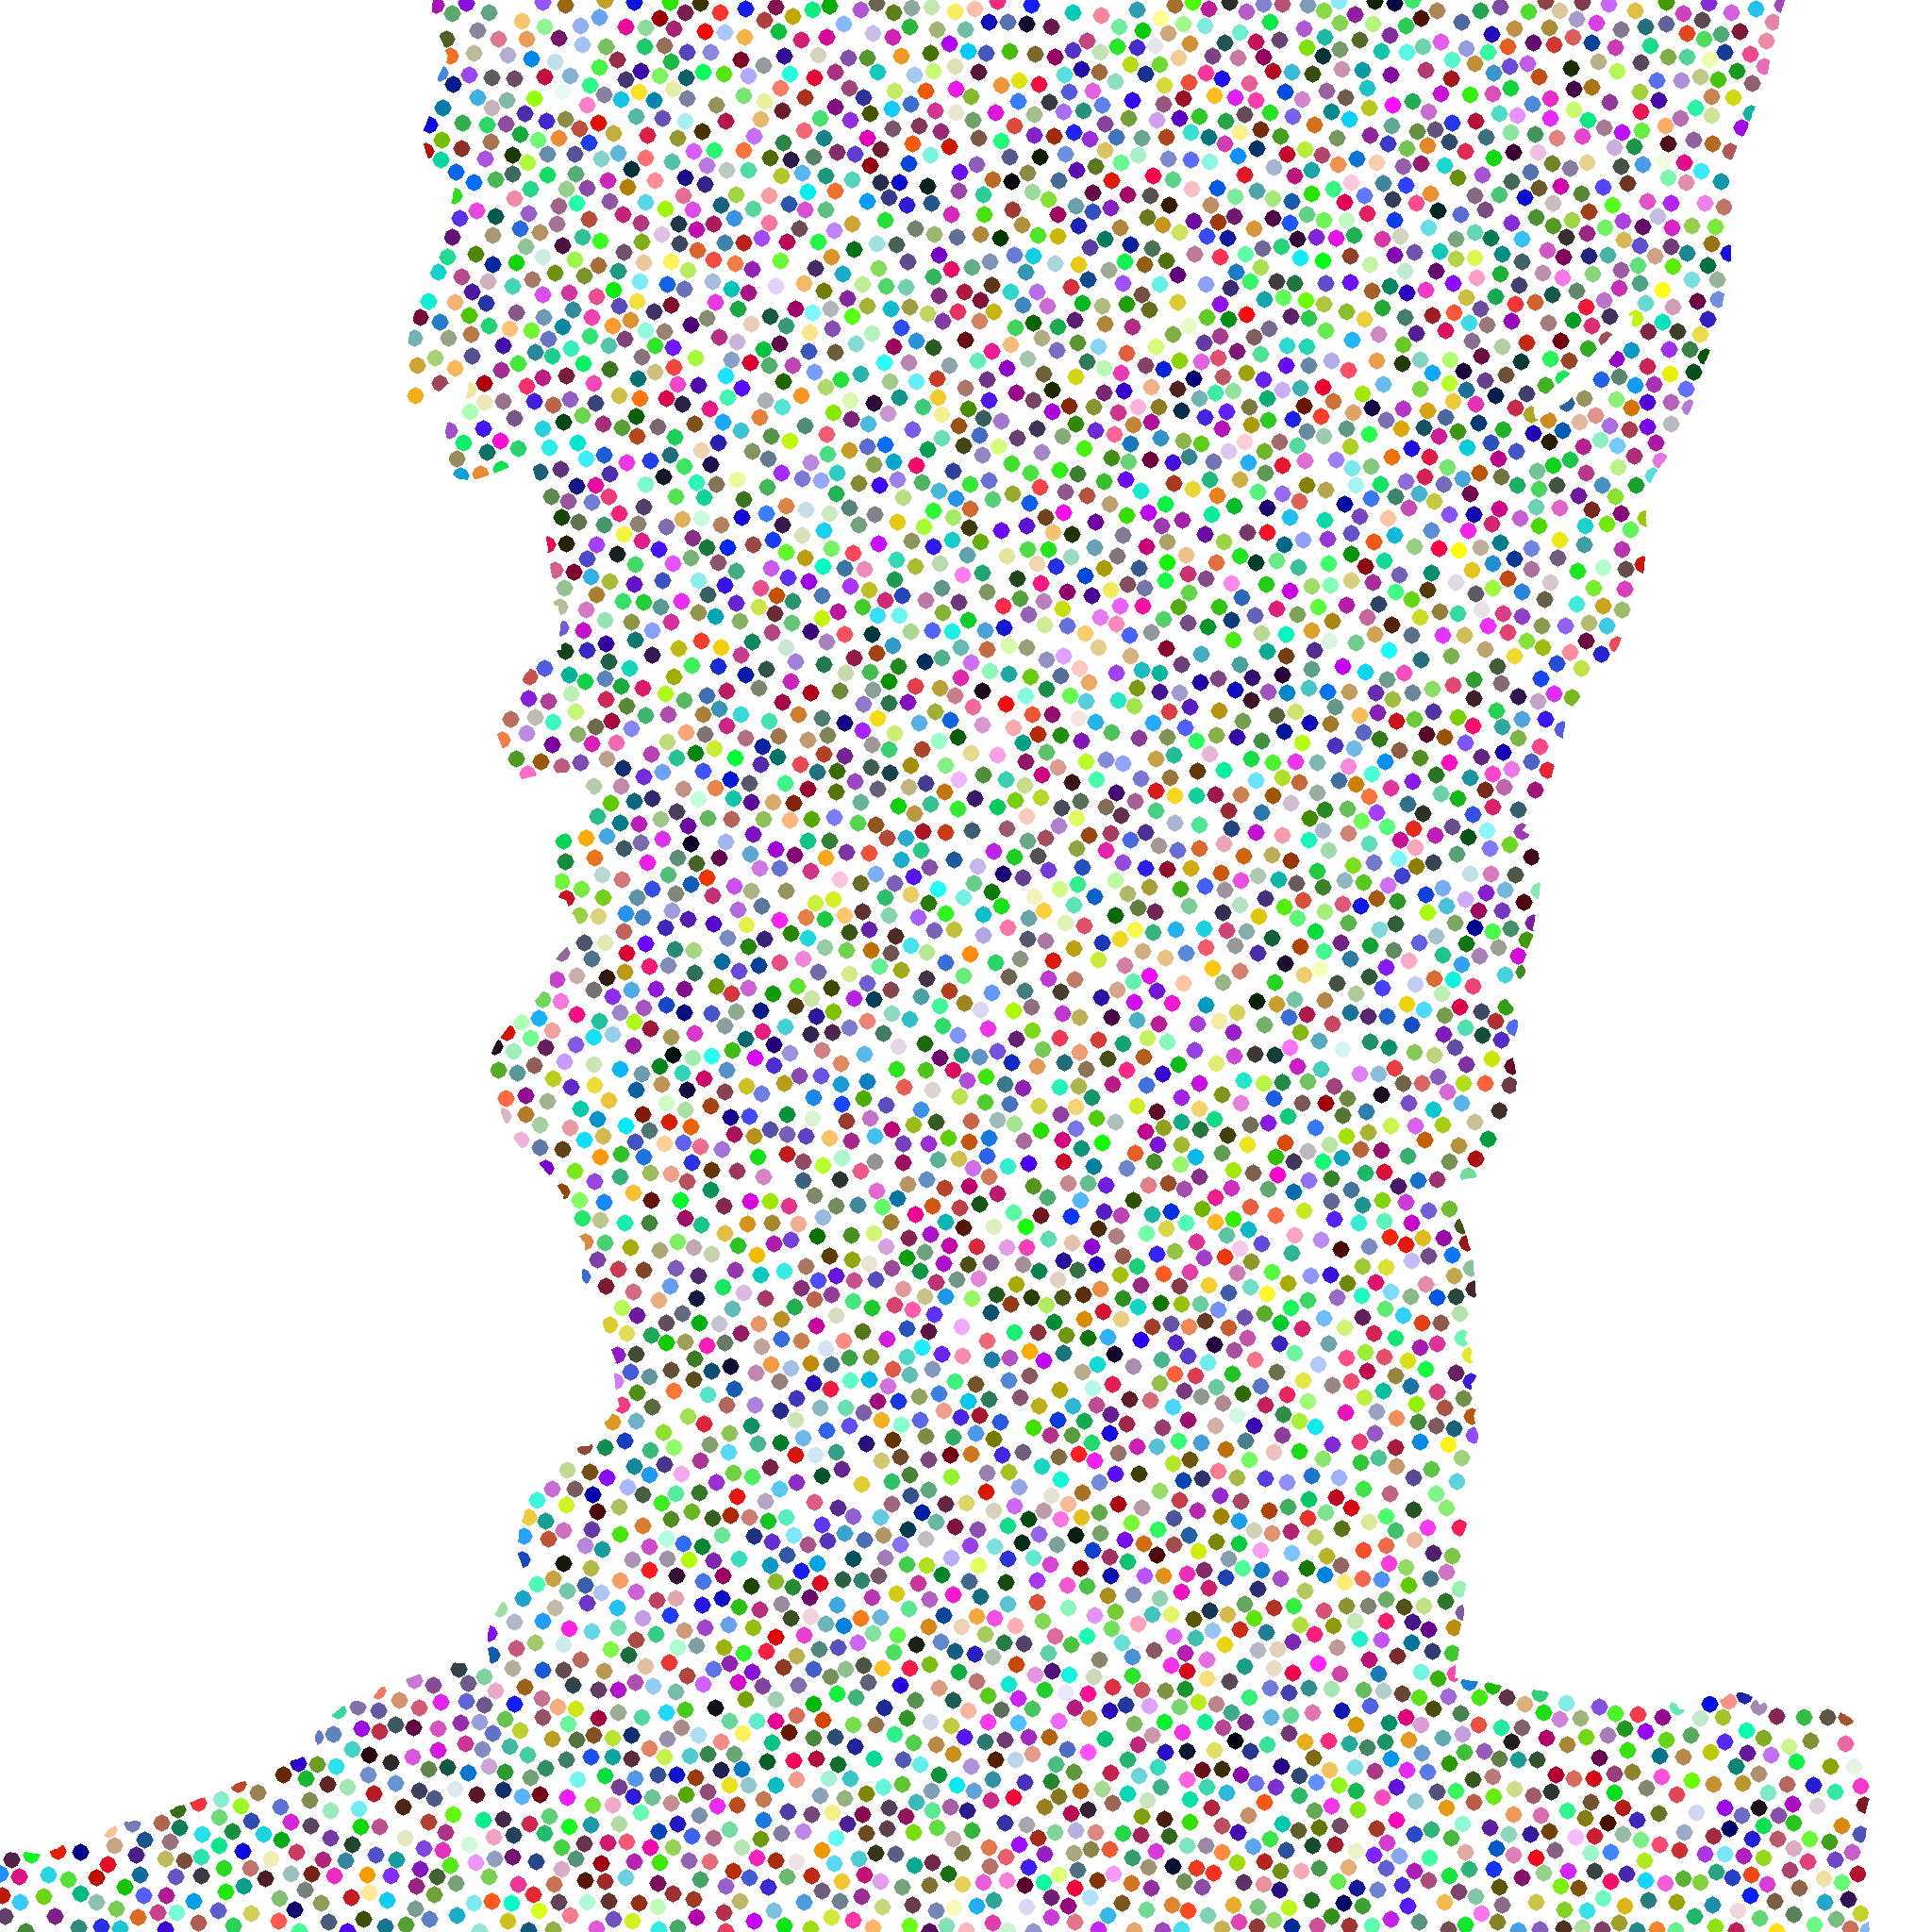
\includegraphics[scale=0.06]{PoissonDisks2D-Garuda}
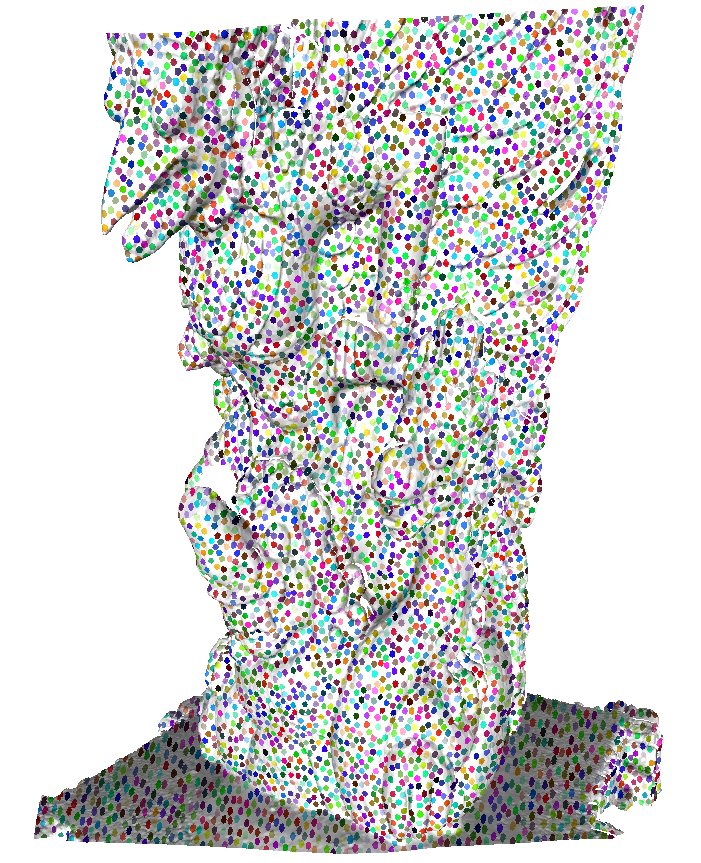
\includegraphics[scale=0.14]{PoissonDisks2DEmbedded-Garuda}
\caption{Poisson-disk sampling of the Garuda model considering disks with an uniform area in 2D. Samples found (a) with their associated disks (b) and the same disks, but embedded in 3D (c)}
\label{fig:poisson_sampling_2d}
\end{figure}

\subsection{Curvature adaptive sampling}
In order to preserve the fine details during the sampling process, it would be interesting to sample more densely the surface areas where the surface curvature is high (representing high changes in the normal field). For this, the idea is to consider the "normalized" Gaussian curvature as probability density function, giving a higher probability to points in areas of high absolute curvature, and a lower probability to points in areas of low absolute curvature.

\arnaud{INSERT GEOMETRIC GAUSSIAN CURVATURE ADAPTIVE SAMPLING}
\arnaud{Subsection incomplete, need an explanation on curvature estimation from the normals (so adding also an explanation on the normal computation using depthmap connectivity and 3D positions)}
